
\begin{frame}{Recap \& Refresh}

        \begin{itemize}
                \item How to build elicited priors
		\item Conjugate priors: normal-normal, poisson-gamma, beta-binomial
		\item Point estimates (mean, mode, median) and HPD credible intervals
		\item Model testing
        \end{itemize}

\end{frame}

\section{Bayesian computation}

\begin{frame}{Intended Learning Outcomes}

        At the end of this day you will be able to:
        \begin{itemize}
		\item describe the use of asymptotic methods,
		\item illustrate the utility of direct and indirect sampling methods,
		\item evaluate the feasibility of Markov Chain Monte Carlo sampling,
                \item implement simple indirect sampling methods in \texttt{R}.
        \end{itemize}

\end{frame}

\frame{
\frametitle{Bayesian computation}

The calculation of posterior distributions often involves the evaluation of complex high-dimensional integrals.\newline

When a conjugate prior is not available or appropriate we can evaluate the posterior distribution with:
\begin{enumerate}
\item asymptotic methods for approximating the posterior density;
\item numerical integration.
\end{enumerate}

}

\frame{
\frametitle{Asymptotic methods}

\begin{block}{Bayesian Central Limit Theorem}
When there are many data points $p(\theta|x)$ will be approximately normally distributed.
\end{block}

For large data points, the posterior can be approximated by a normal distribution with mean equal to the posterior mode and (co)variance (matrix) equal to minus the inverse of the second derivative matrix of the log posterior evaluated at the mode.

}

\frame{
\frametitle{Asymptotic methods}

Example:\newline
Recalling the beta-binomial model with flat prior, $p(\theta|x) \propto \theta^x(1-\theta)^{n-x}$.
\newline

The approximation is given by:
        \begin{enumerate}
        \item take the log: \pause $l(\theta)=x\log\theta+(n-x)\log(1-\theta)$
        \item take the derivative of $l(\theta)$ and set it to zero, obtaining \pause $\hat{\theta}^\pi=\frac{x}{n}$
        \item take the second derivative evaluated at $\hat{\theta}$, obtaining \pause $-\frac{n}{\hat{\theta}}-\frac{n}{1-\hat{\theta}}$
        \item take the minus inverse, obtaining \pause $\frac{\hat{\theta}(1-\hat{\theta})}{n}$ 
        \item $p(\theta|x) \sim N(\hat{\theta}^\pi, \frac{\hat{\theta}(1-\hat{\theta})}{n})$
        \end{enumerate}

}

\begin{frame}{Asymptotic methods}

	\begin{block}{}
		If $p(\theta|x) \propto \theta^x(1-\theta)^{n-x}$ then for large $n$ we have $p(\theta|x) \sim N(\hat{\theta}^\pi, \frac{\hat{\theta}(1-\hat{\theta})}{n})$.
	\end{block}

	Exercise:\\
	$k=20$\\
	$n=100$\\
	$\pi(\theta)=G(1,1)$\\
	Compare the exact and approximated posterior (e.g. use qqplot).\\
	What happens if $n=10$?	

\end{frame}


%%%%%%%%%%%%%%%%%%%%%%%

\frame{
\frametitle{Asymptotic methods}

\textit{Model approximations} or \textit{first order approximations}: the estimate $\theta$ by the mode and the error goes to $0$ at a rate proportional to $1/n$.\newline

The estimates of moments and quantiles may be poor if the posterior differs from normality.\newline

The \textit{Laplace's Method} provides a second order approximation to the posterior mean, with an error that decreases at a rate $1/n^2$.\newline

}


%%%%%%%%%%%%%%%%%%%%%%%

\frame{
\frametitle{Asymptotic methods}

Advantages:
        \begin{itemize}
        \item they replace numerical integration with numerical differentiation,
        \item they are deterministic (without elements of stochasticity).
	\item they reduce the computational complexity if any study of robustness (how sensitive are our conclusions to changes in the prior/likelihood?).
        \end{itemize}

}

%%%%%%%%%%%%%%%%%%%%%%%

\frame{
\frametitle{Asymptotic methods}

Disadvantages:
        \begin{itemize}
        \item they require that the posterior is unimodal,
        \item the require that the size of the data is large (how large is "large enough"?),
        \item for high high-dimensional parameters the calculation of Hessian matrices (second derivatives) are hard.
        \end{itemize}


}

%%%%%%%%%%%%%%%%%%%%%%%

\frame{
\frametitle{Noniterative Monte Carlo methods}

	If ${\theta} \sim h({\theta})$ with $h({\theta})$ being a posterior distribution,
        we wish to estimate $\gamma$, the posterior mean of $c({\theta})$, where $\gamma \equiv E[c({\theta})] = \int c({\theta}) h({\theta}) d{\theta}$.
        
	\vskip 0.5cm

        If ${\theta}_1, {\theta}_2, ..., {\theta}_N$ are independent and identically distributed (iid) as $h({\theta})$, then:
	\pause 
        \begin{equation}
        	\hat{\gamma}=\frac{1}{N}\sum_{i=1}^N c({\theta}_i)
        \end{equation}
	which converges to $E[c({\theta})]$ with probability 1 as $N \rightarrow \infty$.

	\vskip 0.5cm

        The computation of \textbf{posterior expectations} requires only a sample of size $N$ from the posterior distribution.

}

\frame{
\frametitle{Noniterative Monte Carlo methods}

	The variance of $\hat{\gamma}$ can be estimated from the sample variance of the
	$c({\theta}_i)$ values.

	\begin{equation}
    		\hat{se}(\hat{\gamma}) = \sqrt[]{ \frac{1}{N(N-1)} \sum_{i=1}^N [c({\theta_i})-\hat{\gamma}]^2 }
	\end{equation}

	\vskip 0.5cm
	The Central Limit Theorem implies that $\hat{\gamma} \pm 2 \hat{se}(\hat{\gamma})$
	provides the approximated $95\%$ confidence interval.

	$N$ can be chosen as large as necessary to provide a desirable confidence interval.

}

%%%%%%%%%%%%%%%%%%%%%%%

\frame{
\frametitle{Noniterative Monte Carlo methods}

In the univariate case, a histogram of the sampled $\theta_i$ estimates the posterior itself.\newline

An estimate of $p \equiv P\{a<c(\theta)<b\}$ is given by
        \begin{equation}
        	\hat{p} = \frac{\text{number of } c(\theta_i) \in (a,b)}{N}
        \end{equation}

In contrast to asymptotic methods, accuracy improves with $N$, the Monte Carlo sample size (which we can choose and have control upon) rather than $n$ the size of the data set (which can may not be able to control).

}

%%%%%%%%%%%%%%%%%%%%%%%

\frame{
\frametitle{Noniterative Monte Carlo methods}

What happens if we can't directly sample from this distribution?

There are methods for \textbf{indirect} sampling of the posterior distribution: (i) importance sampling, (ii) rejection sampling, (iii) weighted bootstrap.

}

%%%%%%%%%%%%%%%%%%%%%%%

\frame{
\frametitle{Rejection sampling}

If we identify an \textit{envelope function} $g({\theta})$ and a constant $M>0$ such that $L({\theta})\pi({\theta})<Mg({\theta})$ for all ${\theta}$, then:
        \begin{enumerate}
        	\item Generate $\theta_i \sim g(\theta)$,
        	\item Generate $U \sim Uniform(0,1)$,
        	\item If $MUg(\theta_i)<L(\theta_i)\pi(\theta_i)$ accept $\theta_i$ otherwise reject $\theta_i$.
        \end{enumerate}
        
If we repeat this procedure until $N$ samples are obtained, the members of this sample will be random variables from $h(\theta)$.

\begin{block}{}
It is hard to sample from the true posterior but it is easier to sample from the envelope function.
\end{block}

\small{Exercise: approximate a Beta distribution using a uniform envelope function}.

}

%%%%%%%%%%%%%%%%%%%%%%%

\frame{
\frametitle{Markov chain Monte Carlo methods}

\begin{itemize}
\item All previous methods are non-iterative as they draw a sample of fixed size $N$.
\item There is no notion of "convergence" but rather we require $N$ to be sufficiently large.
\item For many problems with high dimensionality it may be difficult to find an importance sampling density or an envelope function.
\end{itemize}

    	In these cases it is now standard practice to use \textit{Markov chain Monte Carlo} (MCMC) methods.

}

%%%%%%%%%%%%%%%%%%%%%%%

\frame{
\frametitle{Markov process and chain}

	\begin{enumerate}
	\item A mathematical object following a stochastic (or random) process, typically defined as a collection of random variables.
	\item The next value of the process depends only on the current value, but it is independent of the previous values.
	\item A Markov chain is a Markov process that has a particular type of state space, which dictates the possible values that a stochastic process can take.
	\end{enumerate}

}

\frame{
\frametitle{Markov chain Monte Carlo}

\begin{block}{Stationary distribution}
The probability distribution to which the process converges for large values of steps, or iterations.
\end{block}

The stationary distribution of an MCMC is the desired posterior distribution.

}

\frame{
\frametitle{Markov chain Monte Carlo}

\begin{itemize}

\item The basic idea is to construct a Markov chain on the state space $\Theta$ whose stationary distribution is the target posterior density $p(\theta|Y)$.

\item We perform a random walk on the state space, so that the fraction of time we spend in each state $\theta$ is proportional to $p(\theta|Y)$. 

\item By drawing correlated samples $\theta_0$, $\theta_1$ , $\theta_2$ , $...$ , from the chain, we can perform Monte Carlo integration with respect to $p(\theta|Y)$.

\end{itemize}

}

\frame{
\frametitle{Markov chain Monte Carlo}

An assessment of \textit{convergence} of the Markov chain to its stationary distribution is required.
\newline

The majority of Bayesian MCMC computation is based on two algorithms: the \textit{Gibbs sampler} and the \textit{Metropolis-Hastings (M-H)} algorithm.

}



%%%%%%%%%%%%%%%%%%%%%%%

\frame{
\frametitle{Gibbs sampler}

	Suppose our model has $k$ parameters ${\theta}=(\theta_1, \theta_2, ..., \theta_k)$.

	\vskip 0.5cm

        We assume that we can sample from the full conditional distributions.

	\vskip 0.5cm

        The collection of full conditional distributions uniquely determines the joint posterior distribution $p({\theta},{y})$ and therefore all marginal posterior distributions $p(\theta_i,\vec{y})$, for $i=1,...,k$.

...

}

%%%%%%%%%%%%%%%%%%%%%%%

\frame{
\frametitle{Gibbs sampler}

...

Given an arbitrary set of starting $\{\theta_2^{(0)}, ..., \theta_k^{(0)}\}$, the algorithm, for $(t=1, ..., T)$, is:
        \begin{itemize}
        \item Draw $\theta_1^{(t)}$ from $p(\theta_1 | \theta_2^{(t-1)}, \theta_3^{(t-1)}, ..., \theta_k^{(t-1)}, {y} )$
        \item Draw $\theta_2^{(t)}$ from $p(\theta_2 | \theta_1^{(t)}, \theta_3^{(t-1)}, ..., \theta_k^{(t-1)}, {y} )$
        \item ...
        \item Draw $\theta_k^{(t)}$ from $p(\theta_k | \theta_1^{(t)}, \theta_2^{(t)}, ..., \theta_{k-1}^{(t)}, {y} )$
        \end{itemize}
    	
        $(\theta_1^{(t)}, \theta_2^{(t)}, ..., \theta_k^{(t)})$ converges to a draw from the true joint posterior distribution $p(\theta_1, \theta_2, ..., \theta_k | {y})$.
        \newline
        
        For $t>t_0$ then $\{{\theta^{(t)}}, t=t_0+1, ..., T\}$ is a correlated sample from the true posterior.

}

%%%%%%%%%%%%%%%%%%%%%%%

\frame{
\frametitle{Gibbs sampler}

\begin{enumerate}
\item The parameter space must be fully \textit{connected}, without "holes".
\item When $\theta$ and $\nu$ are highly correlated the chain will have a "slow mixing".
\item To ensure that all the full conditional distributions are available, the prior distribution of each parameter can be chosen to be conjugate with the corresponding likelihood.
\end{enumerate}

}

%%%%%%%%%%%%%%%%%%%%%%%

\frame{
\frametitle{Gibbs sampler}

A histogram of $\{\theta_i^{(t)}, t=t_0+1, ..., T\}$ provides an estimator of the marginal posterior distribution for $\theta_i$.\newline

The posterior mean can be estimated as the posterior mean:
        \begin{equation}
        	\hat{E}(\theta_i|{y}) = \frac{1}{T-t_0} \sum_{t=t_0+1}^T \theta_i^{(t)}
        \end{equation}
        
The time $0<=t<=t_0$ is called the \textit{burn-in} period.

}

%%%%%%%%%%%%%%%%%%%%%%%

\frame{
\frametitle{Metropolis algorithm}

Given:

\begin{itemize}
	\item $p({\theta}|\vec{y}) \propto h({\theta}) \equiv f({y}|{\theta})\pi({\theta})$
	\item a \textit{candidate}, or \textit{proposal}, symmetric density $q({\theta}^* | {\theta}^{(t-1)})$ which satisfies $q({\theta}^* | {\theta}^{(t-1)})=q({\theta}^{(t-1)} | {\theta}^*)$,
	\item a starting value ${\theta^{(0)}}$ at iteration $t=0$,
\end{itemize}

for $(t=1,..., T)$ the algorithm repeats:

        \begin{enumerate}
        	\item Draw ${\theta}^* = q( \cdot | {\theta}^{(t-1)})$
        	\item Calculate $r=h({\theta}^*)/h({\theta}^{(t-1)})$
        	\item If $r \geq 1$, set ${\theta}^{(t)}={\theta}^*$, otherwise set ${\theta}^{(t)}={\theta}^*$ with probability $r$ or set ${\theta}^{(t)}={\theta}^{(t-1)}$ with probability $1-r$.
        \end{enumerate}
        
        ${\theta}^{(t)}$ converges in distribution to a draw from the true posterior density $p({\theta}|{y})$.


}

%%%%%%%%%%%%%%%%%%%%%%%

\frame{
\frametitle{Metropolis algorithm}

A usual candidate density is:
        \begin{equation}
        	q({\theta}^*|{\theta}^{(t-1)}) = N({\theta}^*|{\theta}^{(t-1)}, \tilde{\Sigma})
        \end{equation}
        
\textit{random walk Metropolis}: symmetric and "self-correcting" distribution.\newline

$\tilde{\Sigma}$, the posterior variance, can be empirically estimated from a preliminary run.

}

%%%%%%%%%%%%%%%%%%%%%%%

\frame{
\frametitle{Metropolis-Hastings algorithm}

When $q({\theta}*|{\theta}^{(t-1)}) \neq q({\theta}^{(t-1)}|{\theta}*)$ the acceptance rate $r$ is:
        \begin{equation}
        r = \frac{ h({\theta}^*) q({\theta}^{(t-1)}|{\theta}^*) }{ h({\theta}^{(t-1)})  q({\theta}^*|{\theta}^{(t-1)})  }
        \end{equation}
        
        A draw ${\theta}^{(t)}$ converges in distribution to a draw from the true posterior density as $t \rightarrow \infty$.

}

%%%%%%%%%%%%%%%%%%%%%%%

\frame{
\frametitle{Hastings independence chain}

If we set $q({\theta}^*|{\theta}^{(t-1)})=q({\theta}^*)$ then the proposal ignores the current value of the variable.\newline

The acceptance rate is:
        \begin{equation}
        r = \frac{h({\theta}^*)/q({\theta}^*)}{h({\theta}^{(t-1)})/q({\theta}^{(t-1)})}
        \end{equation}
        
}

%%%%%%%%%%%%%%%%%%%%%%%

\frame{
\frametitle{MCMC algorithms}

\begin{itemize}
\item \textit{Langevin-Hastings} algorithm introduces a systematic drift in the candidate density.
\item \textit{Slice sampler} algorithm uses auxiliary variables to expand the parameter space.
\item \textit{Hybrid} forms combined multiple algorithm in a single problem.
\item \textit{Adaptive} algorithms use the early output from a chain to refine the sampling as it progresses.
\end{itemize}

}

%%%%%%%%%%%%%%%%%%%%%%%

\frame{
\frametitle{Convergence}

Diagnostic strategy:
        \begin{itemize}
        \item run parallel chains with starting points from a wide distribution;
        \item visually inspect these chains;
        \item for each graph calculate the scale reduction factor;
        \item investigate crosscorrelations among parameters.
        \end{itemize}
        
\begin{figure}[!ht]
		\centering
		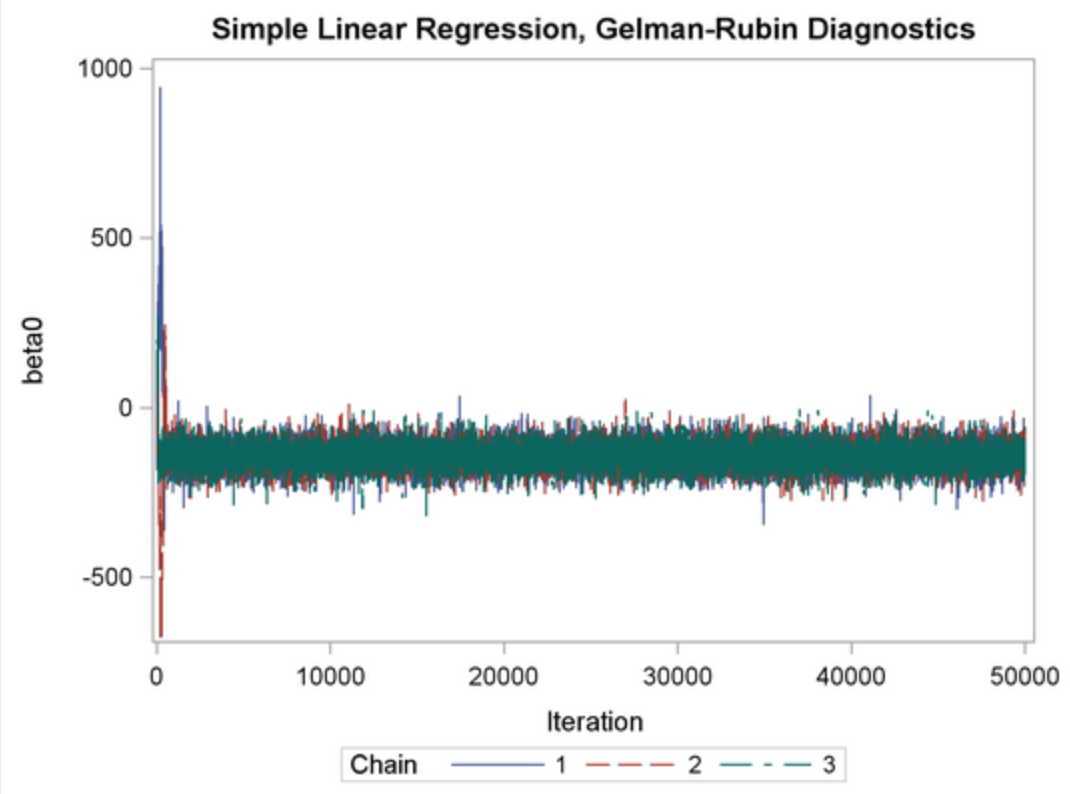
\includegraphics[width=4cm]{Images/Chains.png}
        \caption{Three chains mixing for increasing $t$.}
       	\label{Fig:Chains}
		\end{figure}
}






